\chapter{Introduction into bacterial interactions}
Interactions in natural microbial communities are a very common phenomenon, yet replicating such communities in a controlled environment is challenging, and therefore the impact of such interactions on single species or whole communities is often overlooked. Such interactions are often classified on the basis of their benefits for the respective interacting partners. This thesis describes two projects studying antagonistic interactions, namely antibiotic production and phage-bacteria interactions. 

The first project explores the selection and evolution of antibiotic producers in a microfluidic environment. Here, we modify an existing microfluidic setup to allow for stable production and long-term incubation of microdroplets, containing interacting bacterial communities. The aim of this project is to create a selection mechanism for antibiotic-producing bacteria due to the artificial spatial structure of the microdroplets. In contrast to a well-mixed environment, the benefit of producing an antibiotic is not shared in this case, and therefore, there is a selective advantage for the producing bacteria. 

The second project studies the interactions of phages and bacteria in a spatially structured environment. In this project, we developed a simple reaction-diffusion model to simulate such interactions in an expanding, traveling wave of bacteria and phage together. We observe that phage-resistant bacteria can protect phage-sensitive bacteria in such a wave and can slow down phages expanding while not impairing the spread of phage-sensitive bacteria.

\begin{figure}
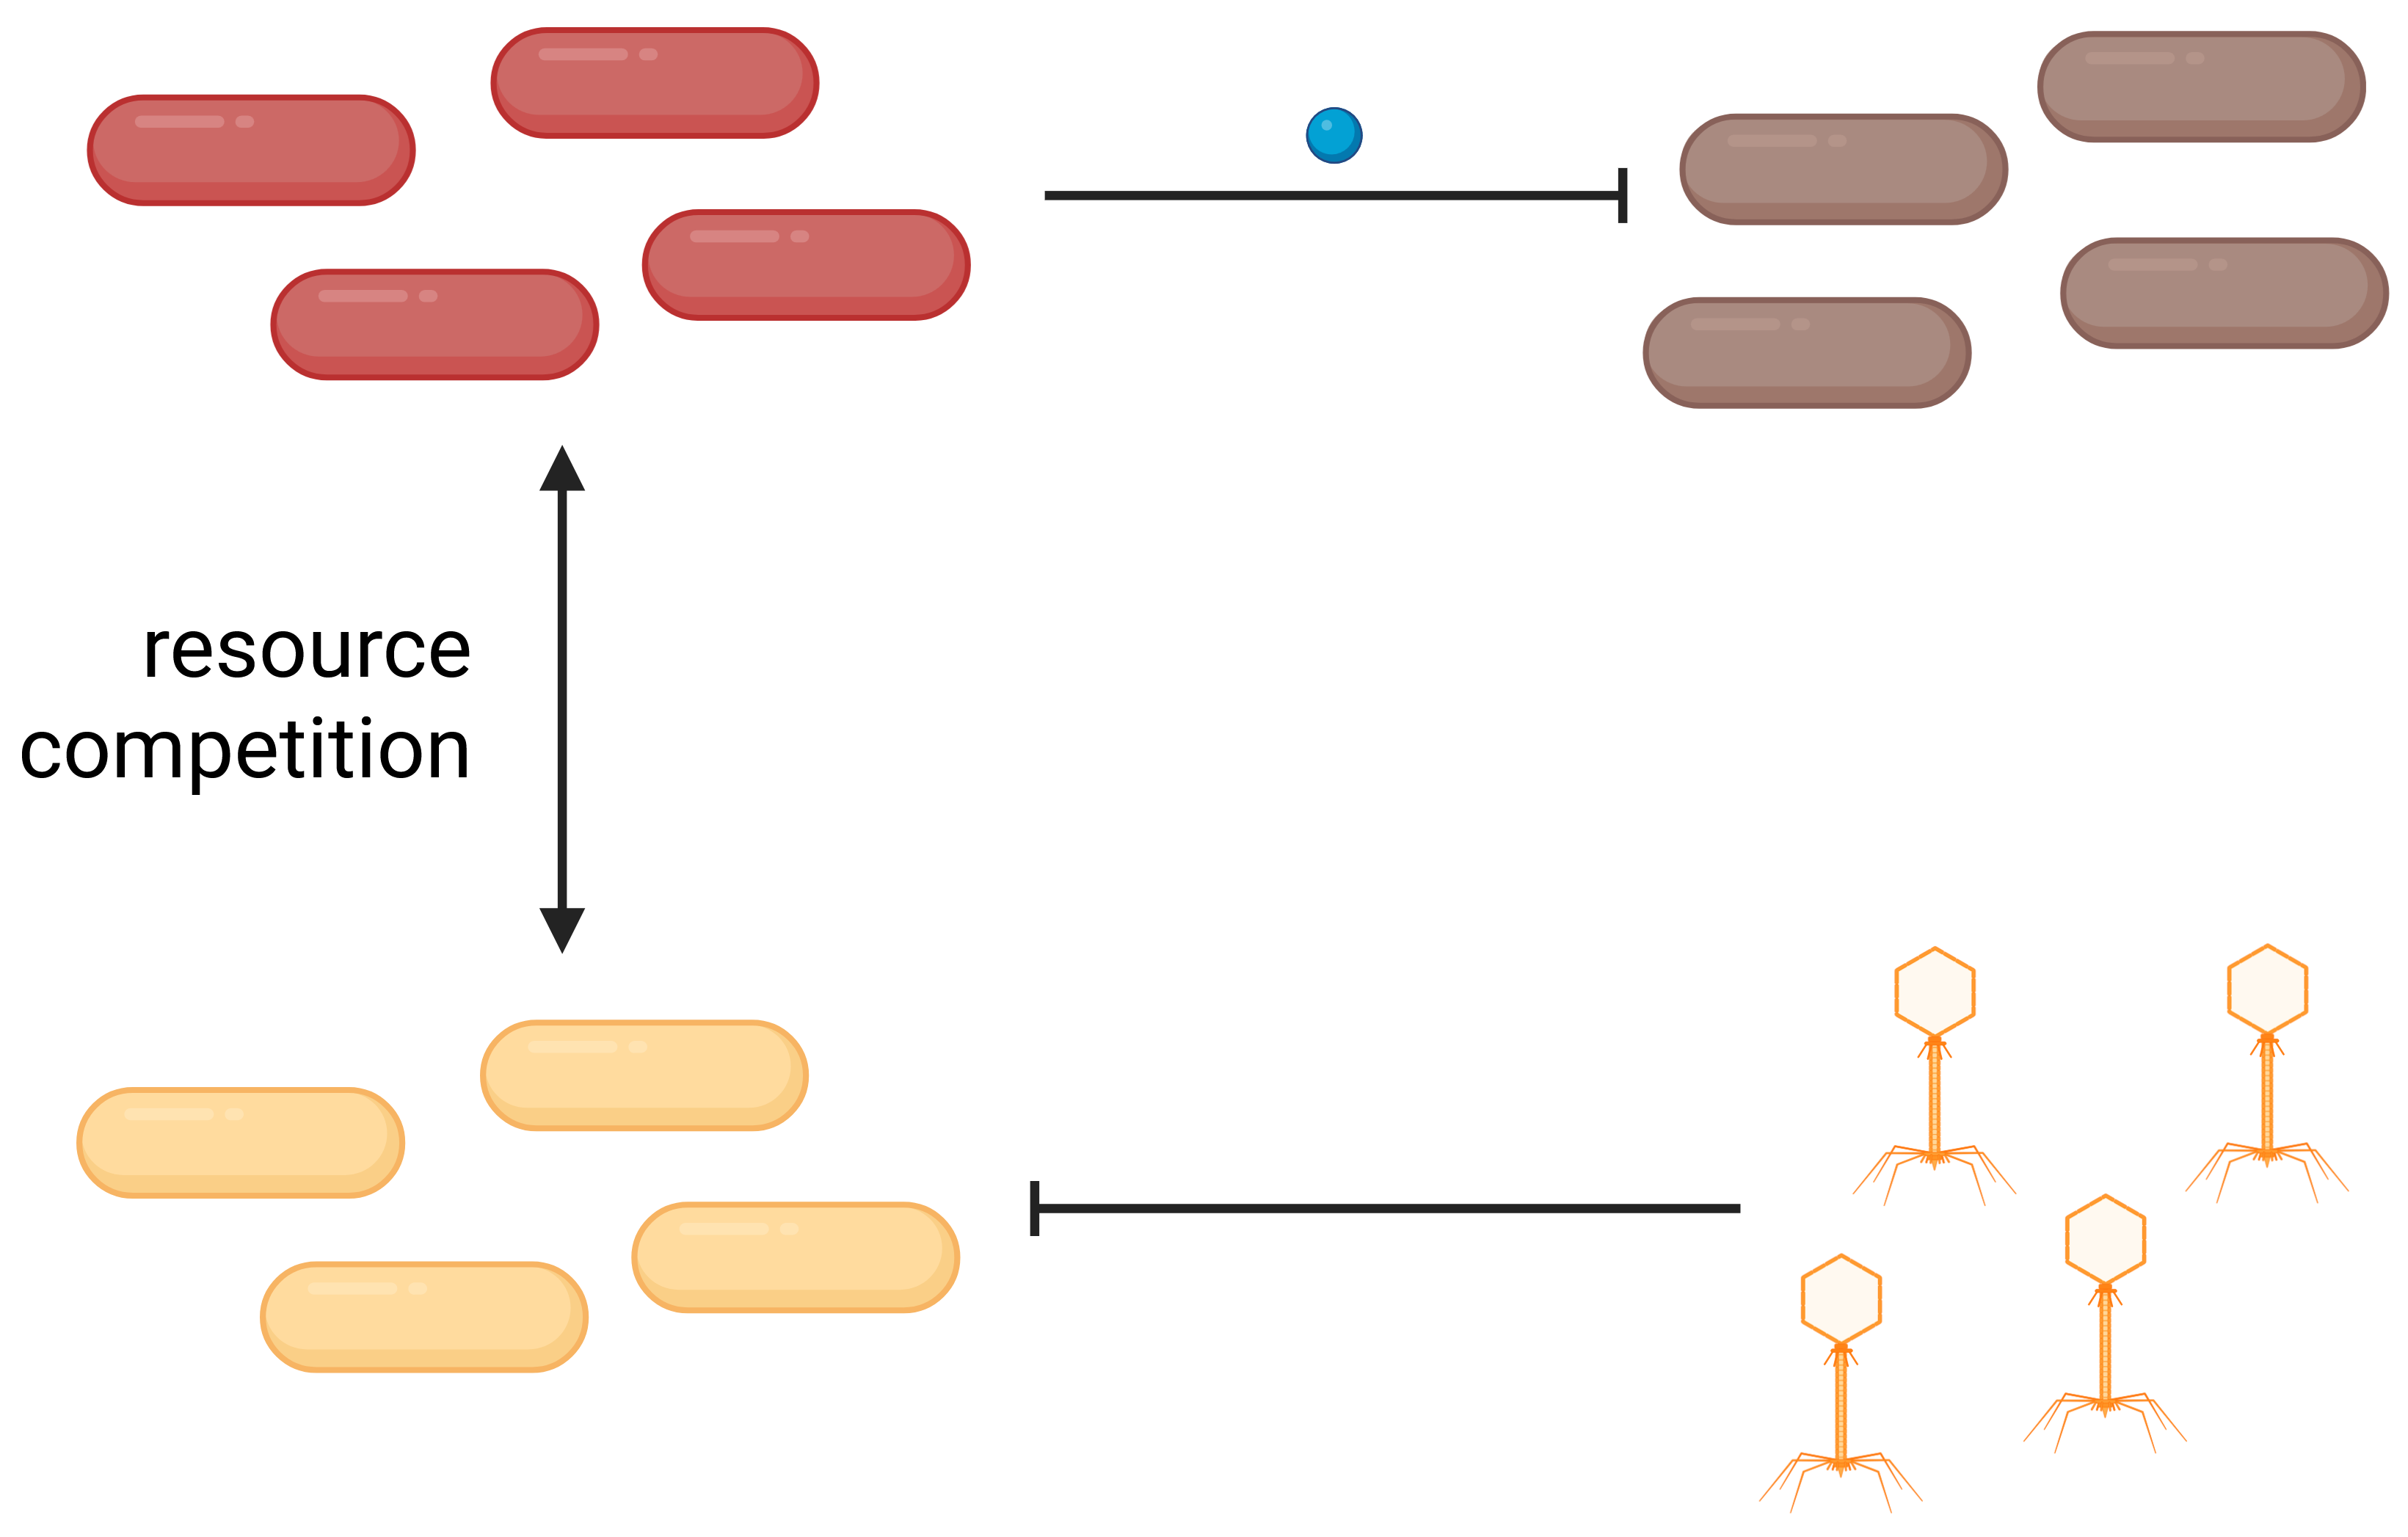
\includegraphics[width=\linewidth]{graphics/2025_09_28_intro_fig1.png}

\caption{\textbf{Antagonistic interactions studied in projects in this thesis}}
\label{fig:intro_shared_interactions}
\end{figure}